\documentclass[10pt]{beamer}

\usetheme[progressbar=frametitle]{metropolis}

\usepackage{booktabs}
\usepackage[scale=2]{ccicons}

\usepackage{pgfplots}
\usepgfplotslibrary{dateplot}

\usepackage{xspace}
\newcommand{\themename}{\textbf{\textsc{metropolis}}\xspace}

\usepackage{tikz}
\usetikzlibrary[topaths]

\usepackage{wasysym}

\title{Popularity, Mixed Matchings, and Self-duality}
\subtitle{Chien-Chung Huang and Telikepalli Kavitha}
\date{\today}
\author{Justin Toth}
\institute{University of Waterloo}
%\titlegraphic{\hfill\includegraphics[height=1.5cm]{logo}}

%Macros
\newcommand{\A}{\mathbb{A}}
\newcommand{\D}{\mathbb{D}} \newcommand{\F}{\mathbb{F}}
\newcommand{\N}{\mathbb{N}} \newcommand{\R}{\mathbb{R}}
 \newcommand{\Z}{\mathbb{Z}}
\newcommand{\Q}{\mathbb{Q}}
 
 
\newcommand{\cA}{\mathcal{A}} \newcommand{\cB}{\mathcal{B}}
\newcommand{\cC}{\mathcal{C}} \newcommand{\cD}{\mathcal{D}}
\newcommand{\cE}{\mathcal{E}} \newcommand{\cF}{\mathcal{F}}
\newcommand{\cG}{\mathcal{G}} \newcommand{\cH}{\mathcal{H}}
\newcommand{\cI}{\mathcal{I}} \newcommand{\cJ}{\mathcal{J}}
\newcommand{\cK}{\mathcal{K}} \newcommand{\cL}{\mathcal{L}}
\newcommand{\cM}{\mathcal{M}} \newcommand{\cN}{\mathcal{N}}
\newcommand{\cO}{\mathcal{O}} \newcommand{\cP}{\mathcal{P}}
\newcommand{\cQ}{\mathcal{Q}} \newcommand{\cR}{\mathcal{R}}
\newcommand{\cS}{\mathcal{S}} \newcommand{\cT}{\mathcal{T}}
\newcommand{\cU}{\mathcal{U}} \newcommand{\cV}{\mathcal{V}}
\newcommand{\cW}{\mathcal{W}} \newcommand{\cX}{\mathcal{X}}
\newcommand{\cY}{\mathcal{Y}} \newcommand{\cZ}{\mathcal{Z}}

\newcommand\numberthis{\addtocounter{equation}{1}\tag{\theequation}}



\newcommand{\size}[1]{\ensuremath{\left|#1\right|}}
\newcommand{\ceil}[1]{\ensuremath{\left\lceil#1\right\rceil}}
\newcommand{\floor}[1]{\ensuremath{\left\lfloor#1\right\rfloor}}

%END MACROS

\begin{document}

\maketitle

\section{Introduction}

\begin{frame}
\frametitle{Voting}
Consider a graph $\alert{G = (V,E)}$, and a matching $\alert{M}$ on $\alert{G}$.

We define the vote of $\alert{u}$ for $\alert{v}$ versus $\alert{v'}$ as
$$vote_u(v,v') = \begin{cases}
1, &\text{if $u$ prefers $v$ to $v'$} \\
-1, &\text{if $u$ prefers $v'$ to $v$} \\
0, &\text{otherwise}
\end{cases}
$$
We can aggregate the margin of victory in an election between two matchings $\alert{M}$ and $\alert{M'}$ by
$$\Delta(M,M') := \sum_{u \in V(G)} vote_u(M(u), M'(u)) $$
where $\alert{M(u)}$ denotes the partner of $\alert{u}$ in $\alert{M}$.
\end{frame}

\begin{frame}
\frametitle{Popular Matchings}
We call $\text{\alert{M}}$ a $\text{\alert{popular}}$ matching if it never loses elections:
$$\forall \text{matchings } M', \quad \Delta(M,M') \geq 0.$$


The max utility popular matching problem $\alert{\text{(MaxPM)}}$ asks to find a popular matching $\alert{M}$ on $\alert{G}$ which maximizes
$$\sum_{e\in M} w(e)$$
for some weights $\alert{ w: E(G) \rightarrow \Q_+}$.
\end{frame}

\begin{frame}
\frametitle{Fractional Matchings}
We can extend this to the fractional matching case:
$$FM_{G} = \{x \in \R^m_+ : x(\delta(u)) \leq 1, \forall u \in V(G)\}$$
By defining for all $\alert{x, y \in FM_{G}}$:
$$\Delta(x,y) = \sum_{u \in V(G)} \sum_{uv, uv' \in \delta(u)} x_{uv}y_{uv'} vote_u(v,v').$$
The polytope of all fractional popular matchings is 
$$P_G := \{x \in FM_{G}: \Delta(x,y) \geq 0, \forall y \in FM_G\}.$$
\end{frame}

\begin{frame}
\frametitle{Mixed Popular Matching Example}
In bipartite graphs, each $\alert{x \in FM_G}$ is a convex combination of matchings. But observe that each $x\in P_G$ need not be a convex combination of popular matchings.
\begin{columns}[T] % align columns
\begin{column}{.48\textwidth}
\begin{figure}
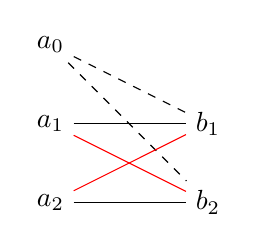
\begin{tikzpicture} 
\node[] (a0) at (0,5) {$a_0$};
    \node[] (a1) at (0,4) {$a_1$};
    \node[] (a2) at (0,3) {$a_2$};
    
    \node[] (b1) at (2,4) {$b_1$};
    \node[] (b2) at (2,3) {$b_2$};
    
    \path[dashed] (a0) edge (b1);
    \path[dashed] (a0) edge (b2);
    \path[-] (a1) edge (b1);
    \path[-] (a2) edge (b2);
    \path[-,red] (a1) edge (b2);
    \path[-,red] (a2) edge (b1);
\end{tikzpicture}
\end{figure}
\end{column}%
\hfill%
\begin{column}{.48\textwidth}
$$ $$
Say each $\alert{a_i}$ has preferences $\alert{b_1 > b_2}$, and each $\alert{b_i}$ has preferences $\alert{a_1 > a_2 > a_0}$.
\end{column}%
\end{columns}


Solid black edges $\alert{S}$ is the only popular matching. If we let $\alert{M}$ be the solid red edges then $$\Pi= \{(S,\frac{1}{2}), (M,\frac{1}{2})\}$$ is a fractional popular matching.
\end{frame}
\section{Integrality of $P_G$ in a special case}

\section{Half-Integrality of $P_G$ in any bipartite instance}
%maybe omit this as next section generalizes and uses same ideas
\section{Half-Integrality of $P_G$ in a roommates instance}

\section{Hardness and Inapproximability}

\section{Open Problems}

\section{Introduction to Stable Matching}
\begin{frame}
\frametitle{Stable Matching Problem}
\begin{overprint}
\onslide<1-3>
Introduced by Gale and Shapley in 1962
\onslide<4-9>
How to solve? Gale Shapley Algorithm:
\onslide<10->
Not very fair to women. Can we do better?
\end{overprint}
\begin{figure}
\centering
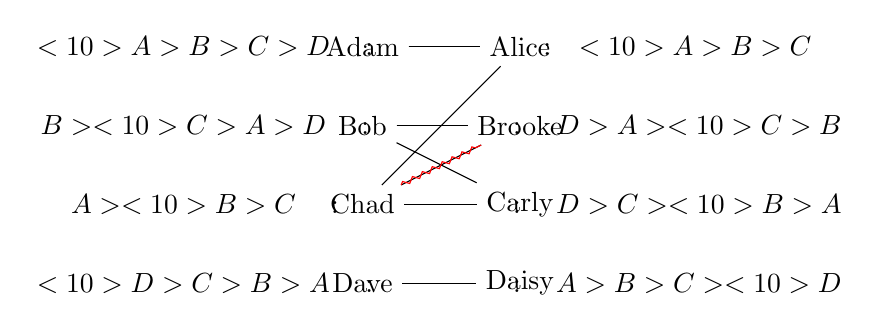
\begin{tikzpicture}
   \node[] (m1) at (0,4) {Adam};
    \node[] (m2) at (0,3) {Bob};
    \node[] (m3) at (0,2) {Chad};
    \node[] (m4) at (0,1) {Dave};
    
    \node[] (w1) at (2,4) {Alice};
    \node[] (w2) at (2,3) {Brooke};
    \node[] (w3) at (2,2) {Carly};
    \node[] (w4) at (2,1) {Daisy};
    
     \node[] () at (-2,4){$\alert<10>{A}>B>C>D\quad:$};
    \node[] () at (-2,3){$B>\alert<10>{C}>A>D\quad:$};
    \node[] () at (-2,2){$A>\alert<10>{B}>C\quad:$};
    \node[] () at (-2,1){$\alert<10>{D}>C>B>A\quad:$};
    
    \node[] () at (4,4){$:\quad \alert<10>{A}>B>C$};
    \node[] () at (4,3){$:\quad D>A>\alert<10>{C}>B$};
    \node[] () at (4,2){$:\quad D>C>\alert<10>{B}>A$};
    \node[] () at (4,1){$:\quad A>B>C>\alert<10>{D}$};
    
    \path[-]<2-3> (m1) edge (w1);
    \path[-]<2-3> (m2) edge (w2);
    \path[-]<2-3> (m3) edge (w3);
    \path[-]<2-3> (m4) edge (w4);
    
    \path[-]<4-> (m1) edge (w1);
    \path[-]<5-7> (m2) edge (w2);
    \path[-]<6> (m3) edge (w1);
    \path[-]<7-> (m3) edge (w2);
    \path[-]<8-> (m2) edge (w3);
    \path[-]<9-> (m4) edge (w4);
    
    
    \path[-,decoration={zigzag,segment length=4,amplitude=.9,
  post=lineto,post length=2pt},color=red]<3> (m3) edge[decorate] (w2);
    
\end{tikzpicture}
\end{figure}
\end{frame}

\begin{frame}
\frametitle{Weighted Stable Matching}
Add weights to pairs to incentivize equitable pairings.\\
Example:
$$c_{\text{Adam,Alice}} = 8$$ since Adam and Alice really like each other,
$$c_{\text{Adam, Carly}} = 2$$ since Adam and Carly don't like each other much.\\
New Goal:
$$\max_{\{\text{Stable Matchings $M$}\}} \sum_{\text{$(m,w)$ Pairs in $M$}} c_{m,w}$$
\end{frame}

\section{Introduction to Linear Programs}

\begin{frame}
\frametitle{What is a Linear Program?}
Let $c, a^1, \dots, a^m \in \mathbb{R}^n$. Let $b \in \mathbb{R}^m$. Find $x \in \mathbb{R}^n$ which satisfies:
\begin{align*}
\max \sum_{i=1}^n c_i x_i&\  &\text{\alert{The Objective Function}}\\
\text{subject to } \sum_{i=1}^n a_i^1 x_i &\geq b_1\\
&\vdots &\text{\alert{The Feasible Region}}\\
\sum_{i=1}^n a_i^m x_i &\geq b_m \\
x &\geq 0
\end{align*}
\end{frame}

\begin{frame}
\frametitle{Polytopes - Geometry of the Feasible Region}
\begin{center}
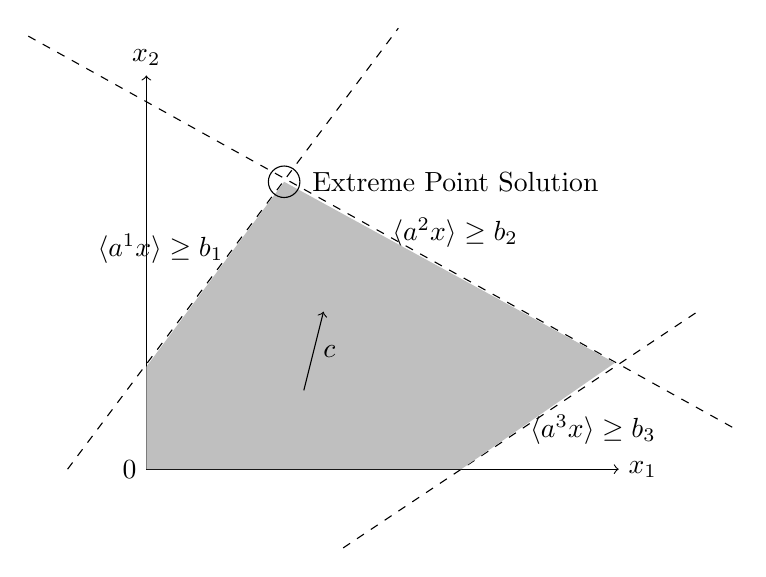
\begin{tikzpicture}
\draw[->] (0,0) node[left]{$0$} -- (0,5)node[above]{$x_2$};
\draw[->] (0,0) -- (6,0) node[right]{$x_1$};

\path[dashed]<1-> (-1,0) edge node[left]{$\langle a^1 x \rangle \geq b_1$} (3.2,5.6);
\path[dashed]<2-> (-1.5,5.5) edge node[right]{$\langle a^2x\rangle \geq b_2$} (7.5,0.5);
\path[dashed]<3-> (2.5,-1) edge node[right]{$\langle a^3 x \rangle \geq b_3$} (7,2);

\path[fill=lightgray]<4-> (0,0) -- (0,1.3) -- (1.75,3.65) -- (5.95,1.35) -- (4,0) -- (0,0);

\path[->] <5-> (2,1) edge node[right]{$c$} (2.25,2);
\draw<6>[] (1.75,3.65) circle (2mm) node[right]{\ \ Extreme Point Solution} ;
\end{tikzpicture}
\end{center}
\end{frame}

\begin{frame}
\frametitle{Why Are Extreme Points Interesting?}
\begin{itemize}
\item We have very efficient algorithms for solving Linear Programs (\alert{Simplex}, \alert{Ellipsoid})
\item These algorithms always give \alert{extreme point} solutions
\item It can be shown that when we can find \alert{optimal solutions} we can always find them at \alert{extreme points}
\end{itemize}
\end{frame}
\section{Formulating Stable Matching as a Linear Program}

\begin{frame}
\frametitle{Incidence Vectors}
We can translate between Matchings and Vectors using \alert{Incidence Vectors} in $\mathbb{R}^E$ indexed by set of all acceptable pairs $E$
\begin{align*}
&\underline{Matching} &\underline{Real\ Vector} \\
&\text{(Adam,Alice)} &x_\text{Adam,Alice} = 1 \\
&\text{(Bob,Carly)} &x_\text{Bob,Carly} = 1\\
&\text{(Chad, Brooke)} &x_\text{Chad, Brooke} = 1\\
&\text{(Dave, Daisy)} &x_\text{Dave, Daisy} = 1 \\
\end{align*}
$x_{m,w} = 0$ for all other pairs $(m,w)$ not in Matching
\end{frame}

\begin{frame}
\frametitle{Rothblum's Formulation}
\begin{align*}
\onslide<1,2->{\max \sum_{\text{Acceptable Pairs } (m,w)} c_{m,w} x_{m,w}}\\
\onslide<1,3->{\text{subject to } \sum_{w \text{ acceptable to } m} x_{m,w} &\leq 1 &\text{For all Men $m$}}\\
\onslide<1,4->{\sum_{m\text{ acceptable to }w} x_{m,w} &\leq 1 &\text{For all Women $w$}} \\
\onslide<1,5->{x_{m,w} + \sum_{\substack{w' \text{ preferred to $w$}\\ \text{by $m$}}} x_{m, w'} + \sum_{\substack{\text{$m'$ preferred to $m$}\\\text{ by $w$}}} x_{m',w} &\geq 1 &\text{For all pairs $(m,w)$}\\}
\onslide<1,6->{1 \geq x &\geq 0}
\end{align*}
\end{frame}

\begin{frame}
\frametitle{Are Extreme Points Incidence Vectors?}
\begin{itemize}
\item We know $0$-$1$ solutions to our Linear Program are Stable Matchings
\item But what if our LP Solver gives an extreme point solution with \alert{$X_{m,w} = \frac{1}{2}$}?
\item We need to show that this cannot happen
\end{itemize}
\end{frame}

\section{Locality Technique}
\begin{frame}
\frametitle{Locality Proof Strategy}
We argue by contradiction:
\begin{enumerate}
\item Start with a minimal counterexample
\item \alert<2>{Show that your fractional extreme point has a $0$ or a $1$}
\item Drop the $0$ or $1$ variable and use minimality to find a contradiction in the smaller problem
\end{enumerate}
\end{frame}

\begin{frame}
\frametitle{Proof Highlights - Finding a $0$ or $1$}
\alert{Rank Lemma:} ``For extreme point $x$, $0 < x < 1$, the maximum number of linearly independent constraints satisfied at equality equals the number of variables."\\
Will contradict with \alert{Token Argument:}
\begin{figure}
\centering
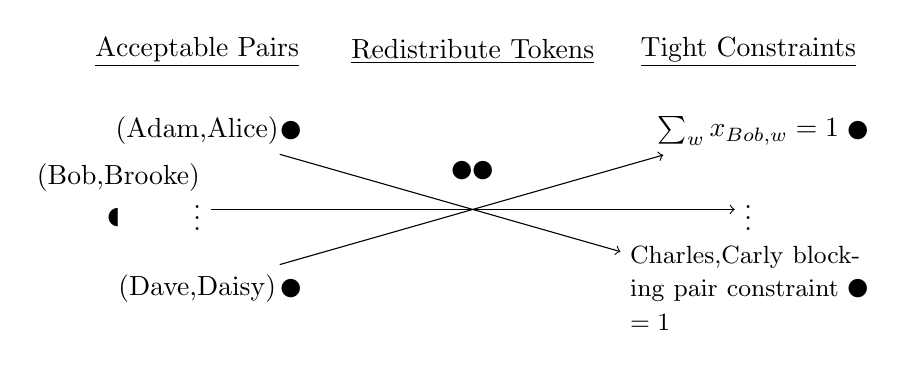
\begin{tikzpicture}
\node[]() at (0,5){\underline{Acceptable Pairs}};
\node[](a1) at (0,4){(Adam,Alice)};
\node<2>[]() at (1.2,4){$\CIRCLE$};
\node[](a2)at(0,3) {$\vdots$};
\node[](a3) at (0,2){(Dave,Daisy)};
\node<2>[]() at (1.2,2){$\CIRCLE$};

\node[]() at (3.5,5){\underline{Redistribute Tokens}};

\node[]() at (7,5){\underline{Tight Constraints}};
\node[](b1) at (7,4){$\sum_{w} x_{Bob,w} = 1$};
\node[](b2) at (7,3){$\vdots$};
\node[text width = 3cm](b3) at (7,2){\small Charles,Carly blocking pair constraint $=1$};

\path[->] (a1) edge (b3);
\path[->] (a2) edge  (b2);
\path[->] (a3) edge (b1);

\node<3>[]() at (3.5, 3.5){$\CIRCLE$$\CIRCLE$};

\node<4->[]() at (8.4, 4){$\CIRCLE$};
\node<4->[]() at (8.4, 2){$\CIRCLE$};

\node<5>[]() at (-1, 3.4){(Bob,Brooke)};
\node<5>[]() at (-1,2.9){$\LEFTCIRCLE$};
\end{tikzpicture}
\end{figure}
\end{frame}

\begin{frame}
\frametitle{Proof Highlights - Token Rules We Used}
Any given acceptable pair $(m,w)$ redistributes its token as follows:
\begin{enumerate}
\item \small If the constraint $$x_{m,w} + \sum_{\substack{w' \text{ preferred to $w$}\\ \text{by $m$}}} x_{m, w'} + \sum_{\substack{\text{$m'$ preferred to $m$}\\\text{ by $w$}}} x_{m',w} \geq 1$$
is tight, give it the token.
\item \small Otherwise
\begin{itemize}
\item If the constraint
$$\sum_{w \text{ acceptable to } m} x_{m,w} \leq 1 $$
is tight, give it $\frac{1}{2}$ a token.
\item \small If the constraint 
$$ \sum_{m \text{ acceptable to } w} x_{m,w} \leq 1$$
is tight, give it $\frac{1}{2}$ a token.
\end{itemize}
\end{enumerate}
\end{frame}

\begin{frame}
\frametitle{Locality Proof Strategy}
We argue by contradiction:
\begin{enumerate}
\item Start with a minimal counterexample
\item \alert<1>{Show that your fractional extreme point has a $0$ or a $1$}
\item \alert<2>{Drop the $0$ or $1$ variable and use minimality to find a contradiction in the smaller problem}
\end{enumerate}
\end{frame}

\begin{frame}
\frametitle{Proof Highlights - Dropping $0$ Variable}

\begin{overprint}
\onslide<1-3>
\alert{Case:} We have $(m,w)$ with $x_{m,w} = 0$ \\
LP for smaller problem:
\onslide<4->
\alert{Lemma:} Assigning all men (or women) favourite partner among two Stable Matchings gives a Stable Matching!
\end{overprint}
\begin{figure}[h]
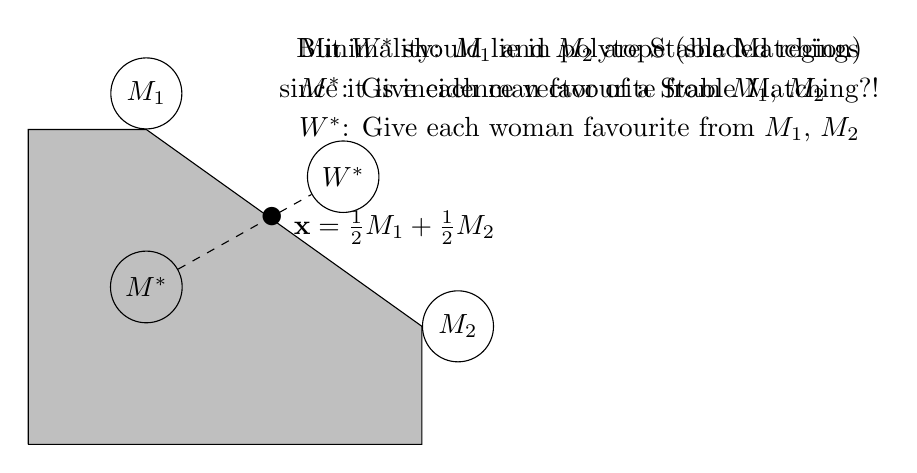
\begin{tikzpicture}


\draw[fill=lightgray] (0,0) -- (0,4) -- (1.5,4)node[above, shape=circle, draw=black]{$M_1$} --node[right]{$\textbf{x} = \frac{1}{2} M_1 + \frac{1}{2} M_2$} (5,1.5)node[right, shape=circle, draw=black]{$M_2$} -- (5,0) -- (0,0);
\node<1>[]() at (7,5){\ \ \ \ \ \ \ \ \ \ \ \ \ \ \ \ \ \ \ \ \ \ \ \ \ \ \ \ \ \ \ \ \ \ \ \ \ \ \ \ \ \ \ \ \ \ \ \ \ \ \ \ \ \ \ \ \ \ \ \ \ \ \ \ \ \ };
\node<2-4>[]() at (7,5){Minimality: $M_1$ and $M_2$ are Stable Matchings};

\node<3-4>[]() at (6.78,4.5){$M^*$: Give each man favourite from $M_1$, $M_2$};
\node<3-4>[]() at (7,4){$W^*$: Give each woman favourite from $M_1$, $M_2$};

\node<4->[shape=circle, draw=black](M) at (1.5,2){$M^*$};
\node<4->[shape=circle, draw=black](W) at (4,3.4){$W^*$};
\path<4->[dashed] (M) edge (W);

\node[]() at (3.1,2.9){$\CIRCLE$};

\node<5>[]() at (7,5){But $W^*$ should lie in polytope (shaded region)};
\node<5>[]() at (7,4.5){since it is incidence vector of a Stable Matching?!};
\end{tikzpicture}
\caption{Stable Matching Polytope}
\end{figure}
\end{frame}

\begin{frame}
\frametitle{References}
\begin{enumerate}
\item Jochen Könemann, Kanstantsin Pashkovich, and Justin Toth. \alert{"The Power of Locality: An Elementary Integrality Proof of Rothblum's Stable Matching Formulation."} $\textit{arXiv preprint}$ arXiv:1605.04427 (2016).
\item Uriel G. Rothblum. \alert{"Characterization of stable matchings as extreme points of a polytope."} $\textit{Mathematical Programming}$ 54.1-3 (1992): 57-67.
\item Lap Chi Lau, Ramamoorthi Ravi, and Mohit Singh. \alert{Iterative methods in combinatorial optimization}. Vol. 46. $\textit{Cambridge University Press}$, 2011
\end{enumerate}
\end{frame}


\end{document}
